\section{Recommendations}\label{sec:recs}
A fixed schedule's L2 TTE is a poor ranking metric: S12 dies inside its second evening's video call, so a dark
theme moves it by only 1.4\,\% although $E_u/\bar P$ rises by 7.6\,\%. We rank levers on $E_u/\bar P$ of S12 and
on the F6 mean of the typical random day S13, with 90\,\% intervals over 1024 parameter draws (\cref{fig:levers}).

\begin{figure}[t]
  \centering
  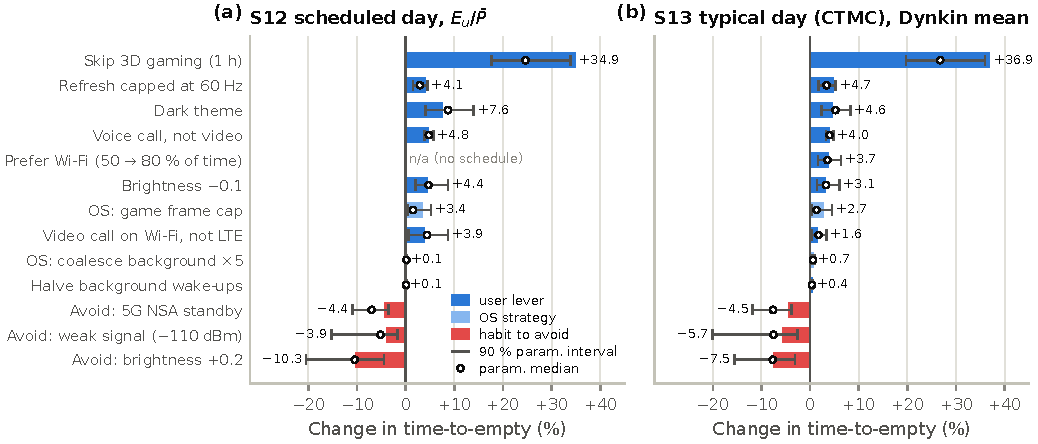
\includegraphics[width=\textwidth]{figures/fig_levers.pdf}
  \caption{TTE change for user levers, OS strategies and habits to avoid on (a) the scheduled and (b) the typical
  random day. Bars: nominal; whiskers: 90\,\% parameter interval; circles: median.}
  \label{fig:levers}
\end{figure}

\subsection{What users can do}
\paragraph{One lever dominates.} Skipping one hour of 3D gaming extends the typical day by 36.9\,\% (median
26.8\,\%, 90\,\%: 19.7--36.0\,\%) and ranks first in every draw; the nominal value is at the top because the
priors throttle harder (median game power 2.59 against 3.12\,W). With uncertain usage rates added the gain spans
5.6--71\,\%. Display and call habits follow at 3--5\,\% each: a 60\,Hz cap $+4.7$\,\% (1.8--5.2), a dark theme
$+4.6$ (2.4--8.3), a voice instead of a video call $+4.0$ (3.3--4.8), Wi-Fi for 80 instead of 50\,\% of the time
$+3.7$ (1.6--6.3) and brightness $-0.1$ $+3.1$ (1.4--6.1); halving background wake-ups gains only 0.4\,\%. Habits
to avoid cost as much: brightness $+0.2$ outdoors $-7.5\,\%$ ($-15.5$ to $-3.1$), weak signal all day $-5.7$
($-20.1$ to $-2.7$), 5G standby without Wi-Fi $-4.5$ ($-11.8$ to $-3.8$). Every gain is positive in at least
98\,\% of the draws and every habit to avoid negative in all.

\paragraph{Scenario-specific advice.} Video over Wi-Fi instead of 5G lasts 32.3 instead of 21.1\,h ($+53\,\%$,
90\,\%: 34--102\,\%), a video call over Wi-Fi instead of LTE 10.8 instead of 6.9\,h, and a voice call 77\,\% longer
than an LTE video call. Standby lasts 443\,h on home Wi-Fi, 378\,h on LTE and 174\,h on 5G with heavy push. At
$-110$\,dBm a social feed loses 12\,\% and a video call 23\,\%. Keeping the phone warm avoids cold shutdowns at
7--44\,\% displayed (\cref{sec:aging}), and a game in a 35\,$^\circ$C car lasts 10.3 instead of 5.7\,h only by
running at 52\,\% performance.

\subsection{What the operating system can do}
\paragraph{O1: a peak-power governor.} Cold, aged phones die from sub-second bursts, not from lack of energy. The
OS can evaluate F4's safe burst $\Delta P_{b,\mathrm{safe}}$ online from voltage, temperature and SOH and cap each
burst at $0.9\,\Delta P_{b,\mathrm{safe}}$, e.g.\ by spreading a CPU boost or a radio promotion over a few
milliseconds; Apple's performance management of aged batteries \cite{AP-BATT} is a rule-based relative. The
stranded charge then stays at or below 2.4\,\% in every cell of the map (\cref{fig:stranded_map}b), and TTE rises
by 7.0\,\% at $-10\,^\circ$C and 25\,\% at $-20\,^\circ$C on the aged pack. The cost is small: the cap binds only in
the last 8.6 and 25\,\% of these runs (below 10.7 and 28.8\,\% displayed), and 97.7 and 92.7\,\% of the requested
burst amplitude is delivered on average. Fixed derating must cut every burst to about a quarter, at all times, to
do as well (\cref{fig:stranded_map}c).

\begin{table}[t]\centering\footnotesize
\caption{OS strategies in the model (25\,$^\circ$C and new pack, except O1 at SOH 0.8; 90\,\% parameter interval
in brackets).}
\label{tab:os}
\setlength{\tabcolsep}{4pt}
\begin{tabularx}{\textwidth}{@{}l>{\raggedright\arraybackslash}p{2.95cm}>{\raggedright\arraybackslash}p{4.0cm}>{\raggedright\arraybackslash}X@{}}
\toprule
\# & Strategy & Change in the model & Effect \\
\midrule
O1 & Peak-power governor & cap bursts at $0.9\,\Delta P_{b,\mathrm{safe}}$ (F4) & stranded 8.5$\to$1.5\,\%
($-10\,^\circ$C), 23.3$\to$2.4\,\% ($-20\,^\circ$C) \\
O2 & Thermal frame cap & game demand $-20\,\%$ & 3.12$\to$2.72\,W; S12 $+3.4\,\%$ [0.4, 5.2], S13
$+2.7\,\%$ [0.3, 4.5] \\
O3 & Tail-aware coalescing & standby bursts $\lambda/5$ \cite{HU12,NA21} & standby $+2.4$/$+25.4$/$+66.7\,\%$
(Wi-Fi/LTE/5G); day $\le0.7\,\%$ \\
O4 & RAT steering & 5G only for bulk \cite{XU20} & avoids $-4.5\,\%$ (5G standby, S13), $-34.7\,\%$ (video on 5G) \\
O5 & Signal-aware deferral & defer bulk at ${<}{-100}$\,dBm \cite{DI13} & avoids $-5.7\,\%$ [$-20.1$, $-2.7$] (S13),
$-12.0\,\%$ (LTE social) \\
O6 & Adaptive refresh & 120\,Hz only to scroll \cite{AT20} & up to $+4.1\,\%$ (S12), $+4.7\,\%$ (S13) \\
O7 & Cold-aware gauge & 0\,\% at $\soc^*(T,\mathrm{SOH},\Delta P_b)$ (F4) & stranded charge within 0.2 points \\
O8 & Time left with a band & state filter, online F6--F7 & ``41\,h (30--54\,h)''; coverage
91\,\% (L0), 88\,\% (L2) \\
O9 & Charging defaults & 80\,\% limit; optimised; JEITA & SOH at 2 years $+1.9$, $+0.76$, $+7.0$ points \\
\bottomrule
\end{tabularx}
\end{table}

\paragraph{Other strategies (\cref{tab:os}).} The frame cap O2 is not free: gaming lasts 13.7\,\% longer, but at
0.78 instead of 0.85 of the requested performance. Coalescing (O3) matters for standby, not for a whole day;
steering (O4) and deferral (O5) avoid losses of 4.5--35\,\%. O7 shows ``X\,\% unavailable until warm'' and, for
30\,s bursts that O1 cannot catch, needs the burst size. The band of O8 covers 91.1\,\% of L0 paths (91.9\,\% from
half charge) but 88.3\,\% of 400 full-model paths, whose mean is 3.8\,\% lower: it needs online re-centring.

\begin{keybox}[A guide for users]
\begin{itemize}
  \item \textbf{Games are the big drain:} one hour of 3D gaming can use a quarter of a day's energy.
  \item \textbf{Prefer Wi-Fi} for video and calls, and in poor coverage; a voice call costs far less than video.
  \item \textbf{Dim a little, use a dark theme and 60\,Hz}: 3--5\,\% each. Less background activity: under 1\,\%.
  \item \textbf{In frost keep the phone in an inner pocket.} An older phone can switch off while still showing
  charge (23\,\% at $-20\,^\circ$C); the charge returns when it is warm.
  \item \textbf{For a long battery life} avoid heat, use the 80\,\% limit or optimised charging, charge
  slowly in the cold.
\end{itemize}
\end{keybox}
